%-----------------------------------------------------
% Chapter: Evaluation
%-----------------------------------------------------
\chapter{Evaluation}
\label{chap:evaluation}
\section{CoVeR Evaluation}
\subsection{Validating Implementation}
\subsubsection{Base Embeddings}
As previously stated, there currently does not exist any public implementation of the CoVeR algorithm. As a basis for validating the quality of the CoVeR model created in this project, the base embeddings generated were compared against embeddings generated using the Glove algorithm. In order to achieve this, a simple framework was set up to compare the the most similar words for each word in both the CoVeR and GloVe embeddings. For this experiment, each model was generated by using a symmetric context window of size 8 and each had a dimensionality of 50. Staying true to both papers, the Adam optimiser was used to train the CoVeR algorithm, whilst the AdaGrad optimiser was used to train GloVe. Both models were trained for 10 epochs. 

\noindent
\newline
To find the most similar words for a given word in both the CoVeR and GloVe model, the cosine similarity measure was used.

\begin{equation}
sim(A, B) =\dfrac{A \cdot B}{\lVert A \rVert \lVert B \rVert}
\end{equation}



\subsubsection{Covariate Specific Embeddings}
The original CoVeR paper validates the quality of the learned covariate weight matrices by clustering. This was done 
\section{Model Evaluations}
\subsection{Language Model}
Typically, language models can be evaluated using either extrinsic or intrinsic methods. Whilst extrinsic evaluation methods measure the performance of a model when applied to an application, intrinsic methods allow for the evaluation of a model independent of any application. A drawback of using extrinsic evaluation is the that it is computationally expensive, as it involves the the full deployment of an application to a task, which then has to be evaluated using 
\subsubsection{Intrinsic Evaluation}
A typical intrinsic evaluation metric used to evaluate a language model is perplexity(REF 19, 30, 43). Perplexity is a measure of how well a given language model will predict test data. The general formula for perplexity is given below

\noindent
\newline
From this 

\begin{figure}[h]
	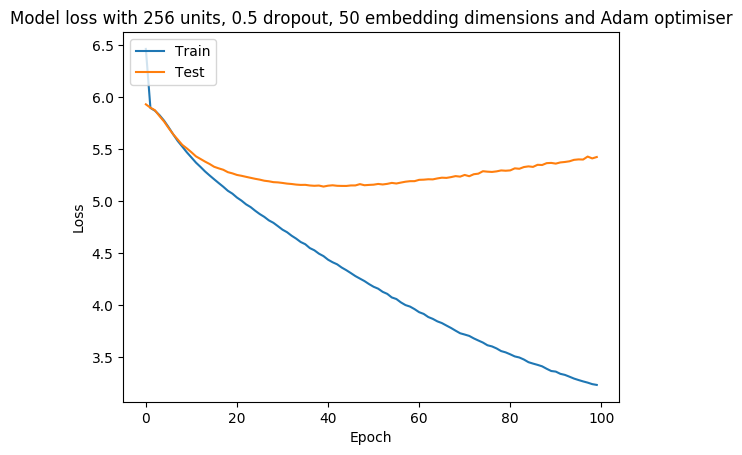
\includegraphics[width=9cm, height=6cm]{./figures/poploss}
	\centering
	\caption{poploss}
	\label{fig:poploss}
\end{figure}

\begin{figure}[h]
	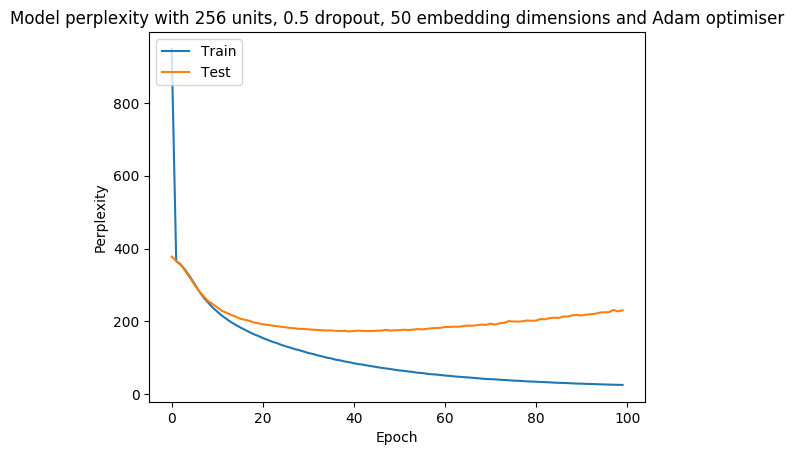
\includegraphics[width=9cm, height=6cm]{./figures/popper}
	\centering
	\caption{popper}
	\label{fig:popper}
\end{figure}

\begin{figure}[h]
	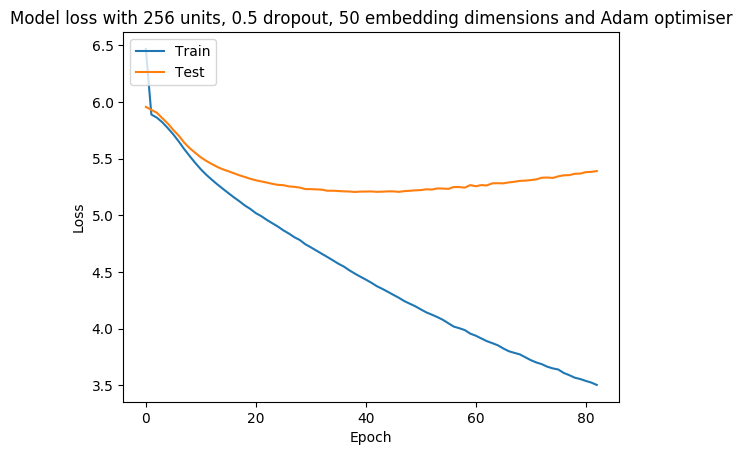
\includegraphics[width=9cm, height=6cm]{./figures/rockloss}
	\centering
	\caption{rockloss.}
	\label{fig:poploss}
\end{figure}

\begin{figure}[h]
	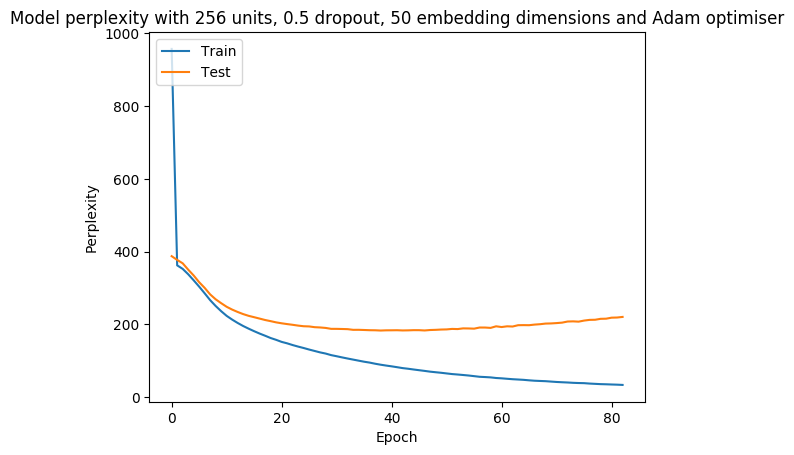
\includegraphics[width=9cm, height=6cm]{./figures/rockper}
	\centering
	\caption{rockper.}
	\label{fig:popper}
\end{figure}

\begin{figure}[h]
	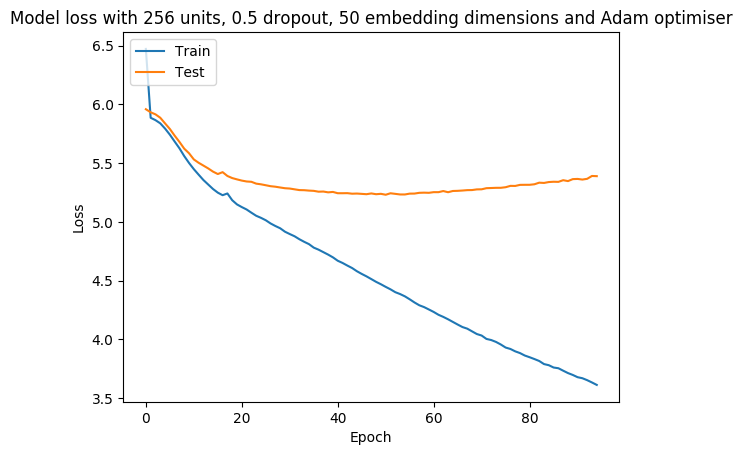
\includegraphics[width=9cm, height=6cm]{./figures/hiphoploss}
	\centering
	\caption{hiphoploss}
	\label{fig:poploss}
\end{figure}

\begin{figure}[h]
	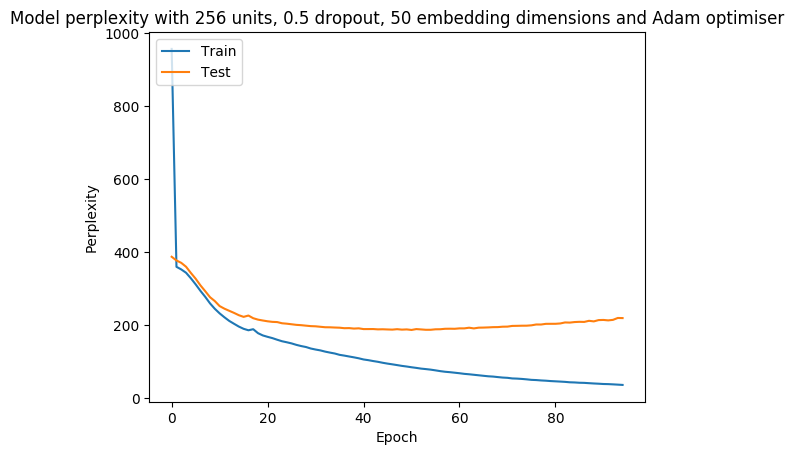
\includegraphics[width=9cm, height=6cm]{./figures/hiphopper}
	\centering
	\caption{hiphopper}
	\label{fig:popper}
\end{figure}

\noindent
\newline


\subsection{Text Classification}
In order to further evaluate the covariate specific word embeddings produced by CoVeR, each covariate embedding was used to train a binary classifier that would discriminate lyrics as either belonging to that particular covariate or not. These were compared with GloVe trained word embeddings to see if the the covaraiets specific word embeddings did indeed capture the semantics of the genre better than generic glove embeddings. The results of the test can be seen in ... below

\begin{table}[ht]
	\centering
	\begin{tabular}{ | p{3cm} | p{2cm} | p{2cm} | p{2cm} | p{2cm} |}
		\hline
		\textbf{Embedding} & \textbf{Training Loss} & \textbf{Training Accuracy} & \textbf{Validation Loss} & \textbf{Validation Accuracy}\\ \hline
		GloVe & 0.5807 & 0.6906 & 0.6194 & 0.6698\\ \hline
		Pop Covariate & 0.5791 & 0.6925 & 0.6122 & 0.6730\\ \hline
	\end{tabular}
	\label{Tab:GlovePopClass}
	\caption{GlovePopClass}
\end{table}

\begin{table}[ht]
	\centering
	\begin{tabular}{ | p{3cm} | p{2cm} | p{2cm} | p{2cm} | p{2cm} |}
		\hline
		\textbf{Embedding} & \textbf{Training Loss} & \textbf{Training Accuracy} & \textbf{Validation Loss} & \textbf{Validation Accuracy}\\ \hline
		GloVe & 0.5251 & 0.7238 & 0.5691 & 0.6985\\ \hline
		Rock Covariate & 0.5200 & 0.7260 & 0.5646 & 0.7009\\ \hline
	\end{tabular}
	\label{Tab:GloveRockClass}
	\caption{GloveRockClass}
\end{table}

\begin{table}[ht]
	\centering
	\begin{tabular}{ | p{3cm} | p{2cm} | p{2cm} | p{2cm} | p{2cm} |}
		\hline
		\textbf{Embedding} & \textbf{Training Loss} & \textbf{Training Accuracy} & \textbf{Validation Loss} & \textbf{Validation Accuracy}\\ \hline
		GloVe & 0.4511 & 0.7926 & 0.5115 & 0.7760\\ \hline
		Hip Hop Covariate & 0.4593 & 0.7878 & 0.4985 & 0.7823\\ \hline
	\end{tabular}
	\label{Tab:GloveHipHopClass}
	\caption{GloveHipHopClass}
\end{table}
\section{SONGIFAI}
\subsection{Requirements Evaluation}
